\chapter{SVM equivalency}
\label{chap:app:svm_link}

For a time series $\textbf{x}_i$, we define the set of pairs $\textbf{X}_{pi}=\{(\textbf{x}_{ij},y_{ij}) \text{ s.t. } j\rightsquigarrow i \text{ or } y_{ij}=+1\}$. It corresponds for a time series $\textbf{x}_i$ to the set of pairs with target samples $\textbf{x}_j$ ($k$ nearest samples of same labels $j\rightsquigarrow i$) or samples $\textbf{x}_l$ that has a different label from $\textbf{x}_i$ ($y_l \neq y_i$) . Identity pairs $\textbf{x}_{ii}$ are not considered. We refer to $\textbf{X}_{p}=\bigcup\limits_{i} \textbf{X}_{pi}$ and consider the following standard soft-margin weighted {\sc svm} problem on $\textbf{X}_p$ \footnote{the {\sc svm} formulation below divides the loss part into two terms similarly to asymetric {\sc svm}}: 
\begin{equation}
\begin{aligned}
&\displaystyle \argmin_{\textbf{w},b,\xi} 
\left\lbrace \frac{1}{2}||\textbf{w}||_2^2
+ C \sum\limits_{i,j,y_{ij=-1}}p_i^-\xi_{ij}
+ C \sum\limits_{i,j, y_{ij=+1}}p_i^+\xi_{ij} \right\rbrace \\
& \text{s.t.  }  y_{ij}(\textbf{w}^T\textbf{x}_{ij}+b) \geq 1-\xi_{ij}
\end{aligned}
\label{eq:SVMSofMarginProblem}
\end{equation}
\noindent where $p_i^-$ and $p_i^+$ are the weight factors for target pairs and pairs of different class.

\noindent  We show in the following that solving the {\sc svm} problem in Eq.~\ref{eq:SVMSofMarginProblem} for $\textbf{w}$ and $b$ solves a similar {\sc mld} problem in Eq.~\ref{eq:MMLPrimalL2} for $D(\textbf{x}_i,\textbf{x}_j)=\frac{1}{2}(\textbf{w}^T\textbf{x}_{ij}+b)$. If we set $p_i^+$ being the half of the number of targets of $\textbf{x}_i$ and $p_i^-$, the half of the number of time series $L$ of a different class than $\textbf{x}_i$:
\begin{align}
	p_i^+ &= \frac{k}{2} = \sum_{j \rightsquigarrow i} \frac{1}{2} \label{eq:pi_plus}\\
	p_i^- &= \frac{L}{2} = \frac{1}{2}\sum_l \frac{1+y_{il}}{2} \label{eq:pi_moins}
\end{align}
% \noindent Note that in the case of $Q$ balanced classes of size $N$,  $p_i^- = N (Q-1)$. 

\subsubsection{Similarities and differences in the constraints}
% \noindent \textbf{Equivalence in the constraints} \\
\noindent First, we recall the {\sc svm} constraints in Eq.~\ref{eq:SVMSofMarginProblem}:
\begin{equation*}
	y_{ij}(\textbf{w}^T\textbf{x}_{ij}+b) \geq 1-\xi_{ij} 
\end{equation*}
\noindent These constraints can be split into two sets of constraints:
%\begin{equation*}
%\begin{aligned}
%y_{ij}(\textbf{w}^T\textbf{x}_{ij}+b) & \geq 1-\xi_{ij} \text{ \quad (same class)} \\
%y_{il}(\textbf{w}^T\textbf{x}_{il}+b) & \geq 1-\xi_{il} \text{ \quad  (different classes)}
%\end{aligned}
%\end{equation*}
%\noindent which is equivalent to:
\begin{equation*}
	\begin{aligned}
		-(\textbf{w}^T\textbf{x}_{ij}+b) & \geq 1-\xi_{ij} \text{ \quad (same class: $y_{ij}=-1$)} \\
		(\textbf{w}^T\textbf{x}_{il}+b) & \geq 1-\xi_{il} \text{ \quad  (different classes: $y_{ij}=+1$)}
	\end{aligned}
\end{equation*}
\noindent By defining $D(\textbf{x}_{ij})=\frac{1}{2}(\textbf{w}^T\textbf{x}_{ij}+b)$, this leads to:
\begin{equation*}
	\begin{aligned}
		-D(\textbf{x}_{ij}) & \geq \frac{1}{2}-\frac{\xi_{ij}}{2} \\
		D(\textbf{x}_{il}) & \geq \frac{1}{2}-\frac{\xi_{il}}{2}
	\end{aligned}
\end{equation*}  
\noindent By summing each constraint two by two, this set of constraints implies the following set of constraints: \\
\resizebox{1\linewidth}{!}{
	\begin{minipage}{\linewidth}
		\begin{eqnarray}
		\begin{cases}
		\bullet \forall i,j,k,l \text{ such that } y_{ij}=-1, \text{ and } y_{kl}=+1, i \neq j \text{ and } i \neq k: \\
		D(\textbf{x}_k,\textbf{x}_l)-D(\textbf{x}_i,\textbf{x}_j) \geq 1-\frac{\xi_{kl}+\xi_{ij}}{2}  \\
		\bullet \forall i,j,l \text{ such that } y_{ij}=-1, \text{ and } y_{il}=+1, i \neq j: \\
		D(\textbf{x}_i,\textbf{x}_l)-D(\textbf{x}_i,\textbf{x}_j) \geq 1-\frac{\xi_{il}+\xi_{ij}}{2}
		\end{cases}
		\label{eq:Rewriten_Constraints}
		\end{eqnarray}
	\end{minipage}
} \\

\noindent By defining $\xi_{ijl}=\frac{\xi_{ij}+\xi_{il}}{2}$, the second constraint in Eq.~\ref{eq:Rewriten_Constraints} from the {\sc mdl} formulation is the same as the constraints in the {\sc svm} formulation in Eq.~\ref{eq:MMLPrimalL2_constraints1}. 

\indent However, an additional set of constraints is present in the {\sc svm} formulation (first set of constraints in Eq.~\ref{eq:Rewriten_Constraints}) and not in the proposed {\sc mld}. Geometrically, this can be interpreted as superposing the neighborhoods of all samples $\textbf{x}_i$, making the union of all of their target sets $\textbf{X}_{pi}$, and then pushing away all imposters $\textbf{x}_{il}$ from this resulting target set. This is therefore creating "artificial imposters" $\textbf{x}_{kl}$ that don't violate the local target space of sample $\textbf{x}_k$, but are still considered as imposters because they invade the target of sample $\textbf{x}_i$ (because of the neighborhoods superposition) (Figure \ref{fig:Neighborhood_scaling_problem}). This is more constraining in the {\sc svm} resolution for the resulting metric $D$ especially if the neighborhoods have different spread. 
% To overcome this issue, we propose to scale all target spheres to 1 in the preprocessing set, such that the risk of over-constraining the problem is very much mitigated.

\begin{figure}[h!]
	\centering
	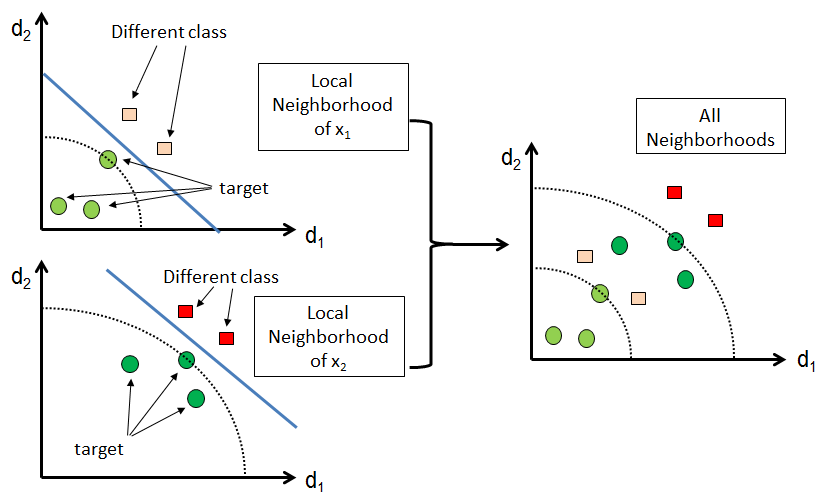
\includegraphics[width=0.8\linewidth]{images/Neighborhood_scaling_problem}
	\caption{Geometric representation of the neighborhood of $k=3$ for two time series $\textbf{x}_1$ and $\textbf{x}_2$ (left). For each neighborhood, time series of different class are represented by a square and the margin by a blue line. Taking each neighborhood separately, the problem is linearly separable ({\sc lp}/{\sc qp} formulation). By combining the two neighborhoods ({\sc svm} formulation), the problem is no more linearly separable and in this example, the time series of different class of $\textbf{x}_1$ (orange square) are "artificial imposters" of $\textbf{x}_2$. }
	\label{fig:Neighborhood_scaling_problem}
\end{figure}


\subsubsection{Similarities and differences in the objective function}
\label{sec:relationship}

% \noindent \textbf{Equivalence in the objective function} \\
\noindent Mathematically, from Eq. \ref{eq:pi_plus}, we write:
%\begin{equation}
\begin{align}
	\sum\limits_{i,l,y_{il=+1}}p_i^+\xi_{il} 
	& = 
	\sum_{il}p_i^+   \frac{1+y_{il}}{2}  \xi_{il} \nonumber\\
	& = 
	\sum_{il} \left( \sum_{j \rightsquigarrow i} \frac{1}{2}\right)  \frac{1+y_{il}}{2}  \xi_{il} \nonumber\\
	& =
	\frac{1}{2}\sum_{i,j \rightsquigarrow i, l} \frac{1+y_{il}}{2}\xi_{il} \label{eq:pi_plus2}
\end{align}
%\end{equation}

\noindent And from Eq. \ref{eq:pi_moins}, we write:
\begin{align}
	\sum\limits_{i,j, y_{ij=-1}}p_i^-\xi_{ij} 
	& = 
	\sum_{i,j \rightsquigarrow i}p_i^-\xi_{ij} \nonumber \\
	& =
	\sum_{i,j \rightsquigarrow i} \left( \frac{1}{2}\sum_l \frac{1+y_{il}}{2} \right) \xi_{ij} \nonumber \\
	& =
	\frac{1}{2}\sum_{i,j \rightsquigarrow i, l} \frac{1+y_{il}}{2}\xi_{ij} \label{eq:pi_moins2}
\end{align}

\noindent By replacing Eqs. \ref{eq:pi_plus2} and \ref{eq:pi_moins2} back into Eq. \ref{eq:SVMSofMarginProblem}, the objective function becomes:
%\begin{equation}
\begin{align}
	&\displaystyle \min_{\textbf{w},\xi} 
	\frac{1}{2}\textbf{w}^T \textbf{w}
	+ C\sum_{i,j \rightsquigarrow i ,l}\frac{1+y_{il}}{2}\frac{\xi_{ij}+\xi_{il}}{2} \nonumber \\
	&\displaystyle \min_{\textbf{w},\xi} 
	\underbrace{ 
		\vphantom{ \sum\limits_{i,j \rightsquigarrow i,l} }
		\frac{1}{2}\textbf{w}^T \textbf{w}
	}_{Regularization}
	+ C \underbrace{
		\sum_{i,j \rightsquigarrow i ,l}
		\frac{1+y_{il}}{2} \xi_{ijl} 
	}_{Loss}
	\label{eq:svm2}
\end{align}	
%\end{equation} 
%\noindent The loss-function part of the {\sc svm} problem is similar to the one in Eq.~\ref{eq:MMLPrimalL2}. We can therefore use such {\sc svm}s with kernels to find non-linear forms for the metric $D$:
%
%\begin{align}
%D(\textbf{x}_{i'},\textbf{x}_{j'}) &= \frac{1}{2} 
%\left( \sum\limits_{ij} \alpha_{ij} 	
%y_{ij} 
%K
%\left( 
%\textbf{x}_{ij}
%,	
%\textbf{x}_{i'j'}
%\right) 
%+ b \right) 
%\label{Eq:nonlinearDSVM}		
%\end{align}

%In this section, we investigate the similarities and the differences between the {\sc lp}/{\sc qp} and {\sc svm} formulations. \\
\indent Even if the loss part (push cost) is the same for both objective functions, the regularization part (pull cost) is different. In the {\sc svm} formulation (Eq. \ref{eq:svm2}), the regularization part tends to minimize the norm of $\textbf{w}$ whereas in {\sc mld} (Eq.~\ref{eq:MMLPrimalL2}), it tends to minimize the norm of $\textbf{w}$ after a linear transformation through $\textbf{X}_{tar}$. This transformation can be interpreted as a Mahalanobis norm in the dissimilarity space with $\textbf{M}=\textbf{X}_{tar}\textbf{X}_{tar}^T$. Nevertheless, both have the same objective: improve the conditioning of the problem by enforcing solutions with small norms. In practice, even with these differences, the {\sc svm} provides suitable solutions for our time series metric learning problem. \\
%($\textbf{X}_{tar}.\textbf{X}_{tar}^T$ can be seen as a specific choice of Tikhonov matrix). 


%%% Local Variables: 
%%% mode: latex
%%% TeX-master: "../roque-phdthesis"
%%% End: 
